\documentclass[../main]{subfiles}

\begin{document}
\chapter{C++11}
\section {Basics}
\subsection{Preprocessor}
\subsubsection{\texttt{\#define} macro}
    When we need to define a very long directive it is possible to break the defined name with \texttt{\textbackslash}.
\begin{Code}
    #define TOTAL_SUM_OF_NUMBERS 12
    #define TOTAL_AMOUNT_OF_NUMBERS 4
    
    #define AVG \
    (TOTAL_SUM_OF_NUMBERS/TOTAL_AM\
    OUNT_OF_NUMBERS)
\end{Code}

\subsubsection{\texttt{\#undef} macro}
    After \texttt{\#undef name} compiler forgets about the \texttt{name}
\begin{Code}
    #include <iostream>
    
    #define VAR 1
    void print()
    {
        /* It is known here */
        std::cout << VAR << std::endl;
    }
    #undef VAR
    
    int main()
    {
        /* Prints "1" */
        print();
        /* Won't compile - VAR isn't known */
        // std::cout << VAR << std::endl;
    }
\end{Code}

\subsubsection{\texttt{\#\#} macro}
    It is an interesting operator which allows one to ,,glue'' two names.
\begin{Code}
    #define JOIN(var1,var2) var1##_##var2
    
    int JOIN(variable,1) = 1;
    
    int main()
    {
        /* Prints "1" */
        std::cout << variable_1 << std::endl;
        
        return 0;
    }
\end{Code}

\subsubsection{\texttt{\#name} macro}
    To print the name of a parameter, we can use the \texttt{\#name} operator. It can be handy during the debugging process
\begin{Code}
    #include <iostream>
    
    #define DEBUG(var) std::cout << #var << std::endl
    
    int main()
    {
        /* Observe that x hasn't been defined! */
        /* Prints "x" */
        DEBUG(x);
        return 0;
    }
\end{Code}

\subsubsection{\texttt{\#error} \textit{text} macro}
    When a compiler meets that directive, it immediately will stop execution and print the \textit{text}.
\begin{Code}
    #define VAR 2
    
    #if (VAR == 1)
        #define COMPILATION_PENDING 1
    #endif
    
    #ifdef COMPILATION_PENDING
        #define COMPILATION_DONE 1
    #else
        /* This will appear in a terminal */
        #error "Compilation corrupted!"
    #endif
\end{Code}

\subsubsection{\texttt{\#include} macro}
    The only missing thing to explain is the difference between \texttt{\#include<...>} and \texttt{\#include "..."}. The former looks for suitable files
in standard directory like \textit{/usr/lib}; the latter will focus on given path.

\subsection{Four types of initialization}
    In C++11 we have four ways to initialize the variable
\begin{Code}
    int value = 1;
    int value (1);
    int value {1};
    int value = {1};
\end{Code}

The last though is a bit different than the others and should be preferred. There are at least a few strong reasons why:

\begin{enumerate}
\item \textbf{Prevents Narrowing Conversions} \\
Brace initialization enforces strict type safety by preventing implicit narrowing conversions (e.g., converting a \texttt{double} to an \texttt{int} or a \texttt{long} to a \texttt{float}).

\begin{Code}
    int a = 3.14;       // Allowed: Truncates to 3
    int b{3.14};        // Error: Narrowing conversion is not allowed
\end{Code}

This helps catch potential bugs at compile time, ensuring that only safe conversions are performed.

\item \textbf{Works for All Types (Consistency)} \\
Brace initialization works for:
\begin{itemize}
    \item Primitive types
    \item User-defined types (classes, structs)
    \item Arrays and STL containers (e.g., \texttt{std::vector}, \texttt{std::initializer\_list})
\end{itemize}

\begin{Code}
    /* Primitive type */
    int x{42};

    /* Object */
    std::string s{"Hello, world"};
    std::vector<int> v{1, 2, 3};
\end{Code}

This uniformity makes it easier to use and read compared to mixing \texttt{=} and \texttt{()} initialization styles.

\item \textbf{Avoids the Most Vexing Parse} \\
Brace initialization avoids the \textbf{most vexing parse}, a situation where the compiler interprets an initialization as a function declaration instead of an object definition.

\begin{Code}
    /* Creates a vector of 10 elements, each initialized to 20 */
    std::vector<int> v1(10, 20);

    /* Could declare a function (!) named v2 that returns vector<int> */
    std::vector<int> v2();
    
    /* All these problems are easily resolved by the braces */
    std::vector<int> v3{10, 20}; 
    std::vector<int> v4{};
\end{Code}

\item \textbf{Supports Initialization Lists} \\
With \{\}, we can initialize objects using an \textbf{initializer list}. This is especially useful for collections or objects with multiple fields.

\begin{Code}
    struct Point {
        int x;
        int y;
    };

    /* Traditional */
    Point p1 = {1, 2};

    /* Uniform initialization */
    Point p2{1, 2};     
\end{Code}

\item \textbf{Better Default Initialization} \\
Brace initialization ensures that objects are \textbf{value-initialized} (initialized to their default values) instead of being left \textbf{uninitialized} or \textbf{undefined}.

\begin{Code}
    /* Uninitialized - could contain garbage value */
    int x;

    /* Value initialized by 0 */
    int y{};
\end{Code}

For classes and structs, this behavior ensures that all fields are initialized correctly.
\end{enumerate}

For these reasons, \{\} is often the best and most robust choice for initialization in C++.

\subsection{Literal type}
    \textbf{Literal types} are the types of \texttt{constexpr} variables and they can be constructed, manipulated, and returned from \texttt{constexpr} functions.
They need to fulfill a few requirements so they need to be one of
\begin{itemize}
    \item possibly \texttt{cv}-qualified \texttt{void} (so that \texttt{constexpr} functions can return \texttt{void}) (since C++14),
    \item scalar type,
    \item reference type,
    \item an array of literal types,
    \item possibly \texttt{cv}-qualified class type that has all of the following properties:
    \begin{itemize}
        \item has a trivial (until C++20) or \texttt{constexpr} (since C++20) destructor,
        \item being one of
        \begin{itemize}
            \item a closure type (since C++17),
            \item an aggregate union type that:
            \begin{itemize}
                \item has no variant members,
                \item has at least one variant member of the non-\texttt{volatile} literal type.
            \end{itemize}
            \item a non-union aggregate type, and each of its anonymous union members:
            \begin{itemize}
                \item has no variant members, or
                \item has at least one variant member of non-\texttt{volatile} literal type.
            \end{itemize}
            \item a type with at least one \texttt{constexpr} (possibly template) constructor that is not a copy or the move constructor.
        \end{itemize}
    \end{itemize}
\end{itemize}

\subsection{Number conversion algorithm}
\begin{enumerate}
    \item If either operand is type \texttt{long double}, the other operand is converted to \texttt{long double}.
    \item Otherwise, if either operand is type \texttt{double}, the other operand is converted to \texttt{double}.
    \item Otherwise, if either operand is type \texttt{float}, the other operand is converted to \texttt{float}.
    \item Otherwise both operands are integrals. If both are signed or unsigned, and one is a lower rank than the other, it is converted to a higher rank.
    \item Otherwise, one operand is signed and one is unsigned. If the unsigned operand is of higher rank the latter is converted to the type of the unsigned operand.
    \item Otherwise, if the signed type can represent all values of the unsigned type, the unsigned operand is converted to the type of the signed type.
    \item Otherwise, both operands are converted to the unsigned version of the signed type.
\end{enumerate}

\subsection{Simple definition of lvalue and rvalue}
    If an object has its name it's lvalue; otherwise, it's rvalue.

\subsection{\texttt{register} and \texttt{volatile}}
    The \textbf{register} variable is similar to automatic variables and exists inside a particular function only. It is supposed to be faster than the local variables.
If a program encounters a register variable, it stores the variable in the processor's register rather than memory if available.\newline

    The \textbf{volatile} variable warns a compiler that the object of that type can change its value without the compiler's knowledge so that the compiler shouldn't rely on
\textit{cache memory} (objects used often can be held in RAM), but it shall take its value directly from the memory where the variable is defined.

\subsection{Comma operator}
    In C++11 comma operator \textbf{,} ensures an order of expression evaluation.
\begin{Code}
    #include <iostream>
    int main()
    {
        int i = 10;
        int j = (i *= 2, i * 20);
        /* Prints "400" */
        std::cout << j << std::endl;

        return 0;
    }
\end{Code}

\subsection{\texttt{constexpr} and \texttt{const}}
\begin{center}
    \begin{tabularx}{\textwidth}{|>{\centering\arraybackslash}X|>{\centering\arraybackslash}X|}
        \hline
        \textbf{\texttt{constexpr}} & \textbf{\texttt{const}} \\
        \hline
        The \texttt{constexpr} value is computed during compilation; & The const value is computed during program execution. \\
        \hline
        The \texttt{constexpr} value can be used in switch/case statements; & Not any const value can be. \\
        \hline
        The \texttt{constexpr} value is safe for multithreading since the value is prepared before program execution; & The const value may not be fully constructed when another thread needs it. \\
        \hline
    \end{tabularx}
\end{center}

\subsection{Storage duration, scope and linkage}
    All information needed is included in the following tables.
    
    \subsubsection{Variable}
        \begin{center}
            \small
            \resizebox{\textwidth}{!}{%
            \begin{tabular}{|c|c|c|c|c|}
                \hline
                \textbf{Type} & \textbf{Declaration} & \textbf{Scope} & \textbf{Storage Duration} & \textbf{Linkage} \\
                \hline
                Local variable & \texttt{int x} & Block & Automatic & None \\
                \hline
                Static local variable & \texttt{static int s\_x} & Block & Static & None \\
                \hline
                Dynamic local variable & \texttt{int* x \{ new int\{\} \}} & Block & Dynamic & None \\
                \hline
                Function parameter & \texttt{void foo(int x);} & Block & Automatic & None \\
                \hline
                External non-constant global variable & \texttt{int g\_x} & Global & Static & External \\
                \hline
                Internal non-constant global variable & \texttt{static int g\_x} & Global & Static & Internal \\
                \hline
                Internal constant global variable & \texttt{constexpr int g\_x \{1\}} & Global & Static & Internal \\
                \hline
                External constant global variable & \texttt{extern const int g\_x \{1\}} & Global & Static & External \\
                \hline
                Inline constant global variable (C++17) & \texttt{inline constexpr int g\_x \{1\}} & Global & Static & External \\
                \hline
            \end{tabular}%
            }
        \end{center}

    \subsubsection{Function}
        \begin{center}
            \small
            \resizebox{\textwidth}{!}{%
            \begin{tabular}{|c|c|c|}
                \hline
                \textbf{Forward declaration type} & \textbf{Example} & \textbf{Notes} \\
                \hline
                Function forward declaration & \texttt{void foo(int x)} & Prototype only, no function body \\
                \hline
                Non-\texttt{const} variable forward declaration & \texttt{extern int g\_x} & Must be uninitialized \\
                \hline
                \textit{const} variable forward declaration & \texttt{extern const int g\_x} & Must be uninitialized \\
                \hline
                The \texttt{constexpr} variable forward declaration & \texttt{extern constexpr int g\_x} & Not allowed, \texttt{constexpr} cannot be forward declared \\
                \hline
            \end{tabular}
            }
        \end{center}

    Thus if we define an object market \texttt{static} inside a function body, this object will keep its value until the next function call.
Static objects are created in the same part of memory as global objects and are zero-initialized by default.

\subsection{Enums}
    Usually, the base type of enumeration is \texttt{int} but there are no contradictions to not do it with any other integral type

\begin{Code}
    enum class CharEnum : char
    {
        Char1,
        Char2,
        Char3
    };
\end{Code}

    Each enumeration has its \textbf{range}, and we can assign any integer value in the range, even if it is not an enumeration value, by using a type cast to the enumeration variable.
For instance
\begin{Code}
    enum Numbers { nfive = -5, two = 2, four = 4, nine = 9};
    Numbers number { static_cast<Numbers>(6) };
\end{Code}
Any enumeration variable doesn't represent 6 but belongs to the range so the assignment is valid.\newline

    To calculate the enumeration range we take the largest enumeration value and find the smallest power of 2 greater than this value and subtract it by one.
In our case, we have $9 < 2^4-1$, so $15$ is the upper end of the range.\newline

    Next, to find the lower limit, we find the smallest evaluation value. If it is non-negative, the lower limit of the range is $0$;
otherwise is negative and we do the same thing as for the upper end of the range but with a minus sign. In our case, we have $-(2^3-1) < -5$ so the lower of the range is $-7$.

\subsection{Unions}
    Some basic information can be found in cppreference. One missing part is that unions can have \texttt{private} and \texttt{public} members, but not \texttt{protected}
as \texttt{union} does not support inheritance.

\section{Pointers and arrays}
    It is platform-dependent which integral type for pointers is used. For instance, one might have a platform for which type \texttt{int} is a 2-byte value and addresses are 4-byte values.

\subsection{Array name and first element pointer}
    An array index starts from 0 since it is not a real index. It just provides information on how many object widths we need to move to get the required one.
Sometimes there is a difference between an array name and the first element address.
\begin{Code}
    #include <iostream>
    
    template <typename T>
    std::size_t size(const T* ptr)
    {
        return sizeof(ptr);
    }
    
    int main()
    {
        const char char_arr[3] { 'a', 'b', 'c' };
        
        /* Prints "Char array size: 3 */
        std::cout << "Char array size: " << sizeof(char_arr) << std::endl;
        
        /* Notice that this number is bigger since it is stored as int type! */
        /* Prints "Pointer size: 8" */
        std::cout << size(char_arr) << std::endl;
        
        const int int_arr[3] { 1, 2, 3 };
        
        /* Prints "Int array size: 12 */
        std::cout << "Int array size: " << sizeof(int_arr) << std::endl;
        
        /* Prints "Pointer size: 8" */
        std::cout << size(int_arr) << std::endl;
    
        return 0;
    }
\end{Code}

\subsection{C-ctrings}
    The \texttt{C-string} is defined as a C-array with chars. It has some corner cases presented on the program below.
\begin{Code}
    #include <iostream>
    
    char arr1[80] {"str"};
    char arr2[80] {'s', 't', 'r'};
    char arr3[] {"str"};
    char arr4[] {'s', 't', 'r'};
    char arr5[] { '%' };
    
    int main()
    {
        /* Prints "str80" */
        std::cout << arr1 << ":" << sizeof(arr1) << std::endl;
        
        /* Prints "str80" */
        std::cout << arr2 << ":" << sizeof(arr2) << std::endl;
        
        /* Prints "str4" */
        std::cout << arr3 << ":" << sizeof(arr3) << std::endl;
    
        /* Maybe prints "str%:3 or something other */
        std::cout << arr4 << ":" << sizeof(arr4) << std::endl;
    }
\end{Code}

Let's discuss the code
\begin{itemize}
    \item \texttt{arr1} is defined as the array of chars with 80 elements. We've used parenthesis initialization, so it's quite obvious
    that all missing elements have been zero-initialized.
    \item \texttt{arr2} is defined differently but also with the initialization list, so that is the same case as before.
    \item \texttt{arr3} hasn't used the explicit number of elements, thus the compiler calculated them itself.
    We've used \texttt{str} and there is a hidden \texttt{\textbackslash0} element, that's why we've got 4 elements.
    \item \texttt{arr4} is the most important case. Here the compiler calculated just three elements,
    without ending \texttt{\textbackslash0}, so when we print it, it won't stop until it finds a random
    \texttt{\textbackslash0} in the memory. The \texttt{\%} sign may appear on the screen (the content of \texttt{arr5})
    if only the compiler puts these two arrays one after another.
\end{itemize}

\subsection{Pointers to multidimensional arrays}
    Let's consider two-dimensional array \texttt{int array2D[4][16]}. This is a table of 4 elements, each of which is a table of 16 elements which means that \texttt{array2D} is the pointer to
the first table of 16 elements, \texttt{array2D + 1} is the pointer to the second table of 16 elements, etc. Let's assume we need to get the value of \texttt{array2D[1][10]}. To achieve that
we need to move to the second element of \texttt{array2D} (array of 16 elements) and then move ten steps to the right in that element. In other words, the whole movement was $(1 * 16) + 10$.
To generalize it - we saw that getting \texttt{array2D[1][10]} required (1 * 16) + 10 movements of \texttt{sizeof(int)} size so it can be deduced that the general equation to achieve the element
\texttt{arr2D[i][j]} is
\begin{equation*}
    step = (i * 10) + j.
\end{equation*}
\noindent
There is no information about the number of rows ([4]) which is redundant for the compiler. It is because a two-dimensional array in the memory is actually flat - the arrangement of elements in memory is not relevant,
the way we move on that memory plays the main role.\newline

    The example above provides the reason why it is redundant to add an array's row number to the array pointer. Therefore these two ways of passing a pointer to a 2D array are equivalent
\begin{Code}
    void read(int ptr[][16]);
    /* 4 is redundant */
    void read(int ptr[4][16]);
\end{Code}
\noindent
It works in the same way for any multidimensional array. It will be easy to remember that we just drop the first ,,dimension''
\begin{Code}
    /* We drop [1] */
    int (*ptr)[2][3][4] = new int [1][2][3][4];
    delete[] ptr;
\end{Code}

\subsection{Pointer with \texttt{mutable} or \texttt{const}}
    There is one possible way that \texttt{mutable} and \texttt{const} can be used together with a pointer.
\begin{Code}
    struct Data
    {
        /* Won't compile */
        // mutable const int i;

        /* Won't compile */
        // mutable int* const ptr;

        /* Okay */
        mutable const int* ptr;
    }
\end{Code}
\noindent
The last expression is possible in use since \texttt{mutable} is related to the pointer which can be modified (only the pointed value is \texttt{const}).

\subsection{\texttt{auto} and reference}
    The \texttt{auto} keyword can introduce some problems in the code when used in the wrong way. The main issue is that \texttt{auto} ,,loses'' information whether an object is \texttt{const} or \texttt{volatile}
and information about referenceness of it.

\begin{Code}
    const int i = 1;
    
    /* j is the copy of i, so there is no information
     * whether j is const or volatile!
     */
    auto j = i;

    double x = 1.0;
    double& x_ref = x;
    
    /* y is a copy of x_ref, so its type is double, not double& */
    auto y = x_ref;
\end{Code}
\noindent
But if we use \texttt{\&} after \texttt{auto} keyword, compiler will add \texttt{const} or \texttt{volatile} to it. This shouldn't be surprise
as changing \texttt{const} object would be a serious violation.
\begin{Code}
    const float& f = 2.0;
    auto& f_ref = f;
    
    /* Compilation error, the compiler added const implicitly */
    f_ref++;
\end{Code}

\subsection{\texttt{auto} and pointers} \label{Auto and pointers}
    Let's start with the observation that \texttt{auto} recognizes whether an object is a pointer or not
\begin{Code}
    int i = 0;
    /* auto knows that &i is the address, so the type of ptr is int* */
    auto ptr = &i;
\end{Code}

To recall, we have three ways of \texttt{const} modifier usage with pointers
\begin{Code}
    int i = 0;
    
    /* ptr1 is the pointer of int type to const int */
    const int* ptr1 = &i;

    /* We cannot modify the value */
    // *ptr1 = 1;

    /* But we can move the pointer */
    ptr1++;

    /* ptr2 is the const pointer of int type to int (we cannot move it) */
    int* const ptr2 = &i;

    /* We can modify the value */
    *ptr2 = 1;  // can modify value

    /* But we cannot move the pointer */
    // ptr2++;

    /* ptr3 is the const pointer of type int to const int */
    const int* const ptr3 = &i;

    /* We neither can modify the value nor move the pointer */
    // *ptr3 = 1;
    // ptr3++;
\end{Code}

    Having the code above we can draw some conclusions
\begin{itemize}
    \item The \texttt{const} qualifier is related to the \textbf{nearest type which stands on its right side} (so \texttt{const int* ptr1 = \&i}
    means that \texttt{const} is related to \texttt{int} \textbf{but not \texttt{int*}!})
    \item If there is no type on the right side, it is related to the \textbf{nearest type which stands on its left side}
    (so \texttt{int* const ptr2 = \&i} means that \texttt{const} is related to \texttt{int*})
\end{itemize}

    That little difference has a huge impact on \texttt{auto}.
Assume that
\begin{Code}
    int i = 0;
\end{Code}
and let's analyze the second example being simpler.\newline

    According to the rules observed above the expression
\begin{Code}
    auto const ptr = &i;
\end{Code}
means \texttt{[$int^{*}$] const ptr} where the type deduced
is \texttt{$int^{*}$} thus we get\linebreak
\textbf{\texttt{auto = $int^{*}$ const}} which is expected behavior.\newline

    Now let's have a look at the first case. According to the rules
\begin{Code}
    const auto ptr = &i;
\end{Code}
means \texttt{const $[int^{*}]$ ptr} but knowing that the \texttt{const}
is related to the \textbf{entire type \texttt{$int^{*}$}} we receive
\textbf{\texttt{auto = $int^{*}$ const}} which is valid expression but
not expected by us.\newline

    The final example is the worst of all - it is a mix of these two -
the below expression has the form of \texttt{const [$int^{*}$] const ptr}
\begin{Code}
    const auto const ptr = &i;
\end{Code}
so a compiler deduces that \textbf{\texttt{auto = $int^{*}$ const}} but
observe that there is one another \texttt{const} after that, so
the code above is interpreted as
\begin{Code}
    int* const const ptr = &i;
\end{Code}
and this, of course, produces the compilation error.\newline

    The fix for this problem is quite simple - \textbf{we need to inform the compiler that the required type is the pointer type,
so just add asterisk after \texttt{auto}, thus \texttt{auto*}}.

\section{Functions}
\subsection{Inline functions}
    To make function \texttt{inline} we need to fulfill at least one of the conditions given below
\begin{itemize}
    \item Declaration or definition (not both!) includes \texttt{inline} keyword.
    \item Function is short (one, two lines) and non-recursive.
    \item Is defined within a class body.
\end{itemize}

\subsection{Default function's arguments}
    As we know, C++ allows the default values of arguments. Here we discuss some restrictions imposed on functions with default arguments.
\begin{itemize}
    \item A compiler will raise an error if it meets the default argument defined twice, so the following implementation won't compile.
    \begin{Code}
        /* File "declaration.h */
        #pragma once
        
        void function(int value = 0);

        
        /* File "main.cpp */
        #include "declaration.h"

        /* error: default argument given for parameter 1 of
         * ‘void function(int)’ [-fpermissive]
         */
        void function(int value = 0) {}
        
        int main()
        {
            return 0;
        }
    \end{Code}

    \item There is an opportunity to repeat the declaration with ,,floating'' default argument
    \begin{Code}
        #include <iostream>
        
        void print(int a, int b, int c, int d = 3);
        void print(int a, int b, int c = 2, int d);
        void print(int a, int b = 1, int c, int d);
        void print(int a = 0, int b, int c, int d);
        
        void print(int a, int b, int c, int d)
        {
            std::cout << a << ":" << b << ":"
                      << c << ":" << d << std::endl;
        }
        
        int main()
        {
            /* Prints "0:1:2:3" */
            print();
            
            /* Prints "5:1:2:3" */
            print(5);

            /* Prints "5:6:2:3 */
            print(5, 6);

            /* Prints "5:6:7:3 */
            print(5, 6, 7);

            /* Prints "5:6:7:8 */
            print(5, 6, 7, 8);
        }
    \end{Code}
    \noindent
    Observe that we cannot swap any two print declarations, for instance
    \begin{Code}
        void print(int a, int b, int c = 2, int d);
        void print(int a, int b, int c, int d = 3);
    \end{Code}
    will produce an error, since \texttt{d} is supposed to have a default value if \texttt{c} has.

    \item Function declaration can appear even in the other function body. In such cases, it hides the main declaration.
    \begin{Code}
        #include <iostream>
        
        void print(int a = 0, int b = 1)
        {
            std::cout << a << ":" << b << std::endl;
        }

        int main()
        {
            /* Internal declaration! */
            void print(int a, int b = 2);

            /* Won't work - the declaration above hides the main one */
            // print();

            /* Prints "0:2" */
            print(0);
            
            return 0;
        }
    \end{Code}

    \item The default argument can be calculated by some other function
    \begin{Code}
        #include <iostream>
        
        int get_arg(int i)
        {
            return i % 2;
        }
        
        void print(int a = 0, int b = get_arg(1))
        {
            std::cout << a << ":" << b << std::endl;
        }
        
        int main()
        {
            /* prints "0:1" (/
            print();
            
            return 0;
        }
    \end{Code}
\end{itemize}

\subsection{General view on function overload resolution}
    \textbf{Overload resolution} includes thee main steps
\begin{enumerate}
    \item Assemble a list of candidate functions. These are functions or template functions that have the same names as the called function.
    \item From the candidate functions, assemble a list of viable functions. These are functions with the correct number of arguments and for which there is an implicit
    conversion sequence, which includes the case of an exact match for each type of actual argument to the type of corresponding formal argument. for example, a function call
    with a type \texttt{float} argument could have that value converted to a \texttt{double} formal parameter, and a template could generate an instantiation for a \texttt{float}.
    \item Determine whether there is a best viable function. If so, you use that function;
    otherwise, the function call is an error. There is a ranking from the best to the worst matching
    \begin{itemize}
        \item Exact match, with regular functions outranking templates.
        \item Conversion by promotion (for instance from \texttt{char} to \texttt{int}).
        \item Conversion by standard conversion (for instance \texttt{long} to \texttt{double}).
        \item User-defined conversions, such as those defined in class declarations.
    \end{itemize}
\end{enumerate}

\noindent
To understand it better, consider the following example
\begin{Code}
    void function(int);                // #1
    float function(float, float = 3);  // #2
    void function(char);               // #3
    char* function(const char*);       // #4
    char function(const char&);        // #5
    
    template <typename T>
    void function(const T&);           // #6
    
    template <typename T>
    void function(T*);                 // #7
    
    int main()
    {
        function('A');
        return 0;
    }
\end{Code}

Let's do it step by step:
\begin{enumerate}
    \item There is nothing to analyze in the first step. All functions above have proper names, so all of them are treated as candidates.
    \item Notice at first, that functions \texttt{\#4} and \texttt{\#7} are not viable because an integral type cannot be implicitly converted to a pointer type.
    \item Now we have five functions to consider. \texttt{\#1} is better than \texttt{\#2} because \texttt{char} to \texttt{int} is promotion and \texttt{char} to \texttt{float} is
    conversion. Functions \texttt{\#3}, \texttt{\#5}, and \texttt{\#6} are better than \texttt{\#1} because they are exact matches but
    \texttt{\#3} and \texttt{\#5} are better than \#6 because they are not templates. So now we have best-two matching functions:
    \texttt{\#3} and \texttt{\#5} which is an error of course.
\end{enumerate}

\subsection{Function mangling and C library}
    C++ mangles a method by emitting the function name, followed by \_\_ , followed by encodings of any method qualifiers (such as \texttt{const}), followed by the mangling of the method's class, followed by the
mangling of the parameters, in order. For example \texttt{Class::function(int, long) const} is mangled as \texttt{function\_\_C3Classil}. This approach, however, leads to problems with importing library functions
from the C language which does not support mangling.\newline

    Assume we want to import the function \texttt{int pow(int value, int exponent)} from some C library in the C++ file. During the compilation, C++ mangles it, and we get something like
\texttt{pow\_\_ii}, but there is no \texttt{int pow\_\_ii(int value, int exponent)} function to import. Due to that C++ provides \texttt{extern "C"} command which disables mangling.
\begin{Code}
    extern "C" pow(int value, int exponent);
\end{Code}
    In case of more than one function declaration, we can use the extended version of it
\begin{Code}
    extern "C"
    {
        int pow(int value, int exponent);
        double pow(double a, int exponent);
    }
\end{Code}
\noindent
or even include the whole C header file
\begin{Code}
    extern "C"
    {
        #include "clib.h"
    }
\end{Code}

\subsection{A \texttt{constexpr} function}
A \texttt{constexpr} function can be called during the compilation phase. In C++11 they are subject to tough restrictions:
\begin{itemize}
    \item a compiler must have the full definition when calling it (the same requirement applies to inline functions),
    \item each argument of \texttt{constexpr} function has to be \texttt{constexpr} (\texttt{const} value or reference to \texttt{constexpr} value),
    \item a result of a \texttt{constepxr} function has to be \texttt{constexpr},
    \item a body of \texttt{constexpr} function can have just one statement - \texttt{return} (thus we cannot have variables defined inside),
    \item a body of \texttt{constexpr} function can't have any loops, conditional, or switch statements except the ternary operator,
    \item a body of \texttt{constexpr} function can have empty instructions, simple declarations, and \texttt{using} directives,
    \item a \texttt{constexpr} function can use global or static variables if only if it doesn't modify them.
\end{itemize}

    In other words, a \texttt{constexpr} function can't have any side effects, so it is \textit{pure functional}. The only possible changes can affect its internal (auxiliary) variables.
\begin{Code}
    constexpr double miles_to_km(double miles)
    {
        return 1.609344 * mile;
    }
    
    int main()
    {
        /* Result "11.265408" is visible in the IDE */
        constexpr double value = miles_to_km(7);
    }
\end{Code}

    Remember that \texttt{constexpr} function will be used by the compiler during the compilation phase if only if an argument will be
\begin{itemize}
    \item explicit constant, for instance, 1, \texttt{str}, etc,
    \item or \texttt{constexpr} object,
    \item or reference to \texttt{constexpr} object.
\end{itemize}
\noindent
If none of these conditions is fulfilled a compiler will call this function at the runtime.

\subsection{The \texttt{noexcept} specifier and operator}
    The \texttt{noexcept} specifier informs a compiler that the function doesn't throw an exception.
\begin{Code}
    /* No guarantee - it can either throw or not */
    void function();

    /* Doesn't throw */
    void function2() noexcept;

    /* Doesn't throw */
    void function3() noexcept(true);

    /* No guarantee - it can either throw or not */
    void function4() noexcept(false);
\end{Code}

    We also have \texttt{noexcept} operator mostly used to check whether a function throws or not. It is important that \textbf{\texttt{noexcept} doesn't invoke a function
so only declaration is needed}.
\begin{Code}
    #include <iostream>
    
    void function1(double) noexcept(true);
    void function2(double);
    
    int main()
    {
        constexpr bool value1 = noexcept (function1(1.0));
        
        /* Prints "1" so true */
        std::cout << value1 << std::endl;
        
        constexpr bool value2 = noexcept (function2(1.0));
        
        /* Prints "0" so false */
        std::cout << value2 << std::endl;
    }
\end{Code}

\subsection{The \texttt{main()} function}
    It is the only function that doesn't need to have a return clause - if it doesn't have it, a compiler will write it by itself in the most simple way
\begin{Code}
    int main()
    {
        /* compiler will add "return 0;" here */
    }
\end{Code}

\subsection{A lambda expression}
    There are most important information about \textbf{lambdas} in C++ 11
\begin{itemize}
    \item \texttt{mutable} allows to modify values passed in captures.
    \item In C++11 a lambda can't have the default parameter values.
    \item A lambda is a functor written outside of any class, so it cannot ,,see'' any internal class members without passing \texttt{this}.
    \item To create recursive lambda we use lambda's capture list
    \begin{Code}
        #include <iostream>
        
        int main()
        {
            /* Pass itself in the capture list */
            const std::function<int(int)> fib = [&fib](int idx)
            {
               if (idx < 0)
               {
                  std::runtime_error("Idx < 0!");
               }
               
               if (idx == 0)
               {
                  return 0;
               }
               
               if (idx == 1)
               {
                  return 1;
               }
               
               return fib(idx - 1) + fib(idx - 2);
            };

            /* Prints "55" */
            std::cout << fib(10) << std::endl;
            
            return 0;
        }
    \end{Code}
    
\end{itemize}

\section{Classes}
\subsection{Constructors and destructors}
    A few important notes about constructors and destructors:
\begin{itemize}
    \item Constructors are not inherited.
    \item It is prohibited to throw an exception from a destructor.
    \item If a given class is the base class, the destructor must be virtual.
    \item If all created objects should have the same initial value of member, we can initialize it directly
    \begin{Code}
        struct Data
        {
            const int value { 5 }; 
        };
    \end{Code}
    \item To catch an exception thrown by the initialization list object, we use a special syntax. It is important to remember that an exception is \textbf{thrown again} no matter if caught or not.
    \
    \begin{Code}
        #include <exception>
        #include <iostream>
        
        struct Throwing
        {
            Throwing()
            {
               throw std::runtime_error("Exception!");
            }
        };
        
        class Initializing
        {
        public:
            Initializing()
               try : m_throwing() // try : catch (...) {}
               {
               }
               catch (std::runtime_error& e)
               {
                  std::cout << "Constructor caught: " << e.what() << std::endl;
                  /* Exception is thrown again here! */
               }
           
        private:
            Throwing m_throwing;
        };
        
        int main()
        {
            try
            {
                Initializing initializing {};
            }
            catch(std::runtime_error& e)
            {
                std::cout << "Exception handled: " << e.what() << std::endl;
            }
            return 0;
        }
    \end{Code}
    \item Constructors can be delegated.
    \item Constructors can be reused from base class via \texttt{using} directive.
\end{itemize}

\subsection{Members initialization}
    When we have a member initializer list that initializes more than one item, the items are initialized in the order in which they were declared, not in the order
in which they appear in the initializer list.
\begin{Code}
    #include <iostream>
    
    struct Data1
    {
        Data1() { std::cout << "Data1 "; }
    };
    
    struct Data2
    {
        Data2() { std::cout << "Data2 "; }
    };
    
    struct Datas
    {
        Datas(): data1 (), data2 ()
        {
        }
        
        Data2 data2;
        Data1 data1;
    };
    
    int main()
    {
        /* Prints "Data2 Data1" not "Data1 Data2" */
        Datas datas {};
        
        return 0;
    }
\end{Code}

\subsection{Special member functions}
    Since C++11 we have six special member functions
\begin{enumerate}
    \item Default constructor,
    \item Copy constructor,
    \item Move constructor,
    \item Copy assignment operator,
    \item Move assignment operator,
    \item Destructor.
\end{enumerate}

    The overview of when special member functions are automatically generated depending on which (other) constructors and special member functions are declared is presented
in the picture
\begin{center}
    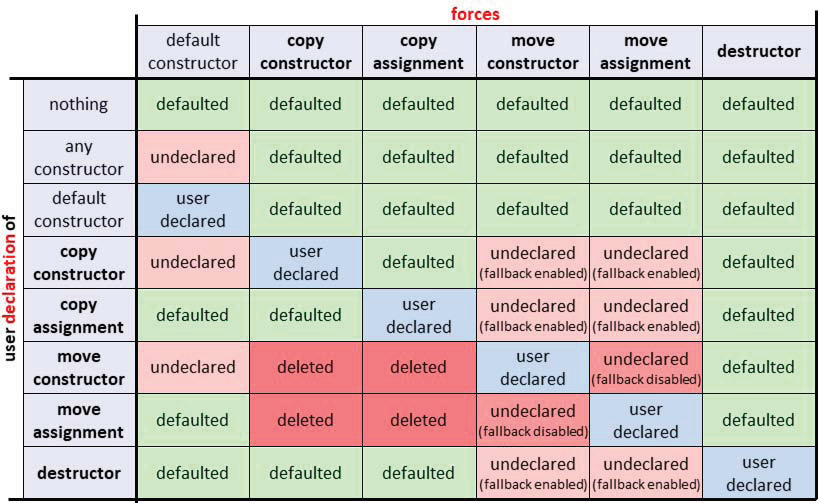
\includegraphics[scale=0.5]{Pictures/specials.png}
\end{center}
\noindent
    The three main things worth mentioning in this table are that
    \begin{itemize}
        \item a default constructor is only declared automatically if no other constructor is explicitly declared.
        \item the custom copying member functions and the destructor disables move support, however, a request to move an object still works because of \textbf{copying as a fallback}.
        \item The custom moving member functions disable copying.
    \end{itemize}

\begin{Code}
    /* Declared copying disables moving but fallback is enabled */
    struct CopyOnly
    {
        CopyOnly() = default;

        /* Or just CopyOnly(const CopyOnly&) = default */
        CopyOnly(const CopyOnly&)
        {
            std::cout << "const CopyOnly& constructor" << std::endl;
        }

        /* Or just CopyOnly& operator=(const CopyOnly&) = default */
        CopyOnly& operator=(const CopyOnly&)
        {
            std::cout << "const CopyOnly& operator=" << std::endl;
            return *this;
        }
    
        /* No special moving functions declared */
    };
    
    /* Declared moving disables copying */
    struct MoveOnly
    {
        MoveOnly() = default;

        /* Or just MoveOnly(MoveOnly&&) = default */
        MoveOnly(MoveOnly&&)
        {
            std::cout << "MoveOnly&& constructor" << std::endl;
        }

        /* Or just MoveOnly& operator=(MoveOnly&&) = default */
        MoveOnly& operator=(MoveOnly&&)
        {
            std::cout << "Move&& operator= called" << std::endl;
            return *this;
        }
        
        /* No special copying functions declared */
    };
    
    int main()
    {
        CopyOnly copy0;
        /* These make a copy due to the fallback */
        CopyOnly copy1 { std::move(copy0) };
        copy0 = std::move(copy1);
    
        MoveOnly move0;
        /* error: use of deleted function
         * ‘constexpr MoveOnly::MoveOnly(const MoveOnly&)’
         */
        // MoveOnly move1 { move0 };  
        
        MoveOnly move1;
        /* error: use of deleted function
         * ‘MoveOnly& MoveOnly::operator=(const MoveOnly&)’
         */
        // move1 = move0;
    
        return 0;
    }
\end{Code}

\subsection{The rule of zero, three and five}
\subsubsection{Rule of zero}
    \textbf{If you can avoid defining any default operation, do it.}

\subsubsection{Rule of three}
    \textbf{Either declare all three: a copy constructor, a copy assignment operator, and a destructor or none of them}.
This rule was applied before the introduction of the C++11 standard.
    
\subsubsection{Rule of five}
    \textbf{Either declare all five: a copy constructor, a move constructor, a copy assignment operator, a move assignment operator and a destructor or none of them}.
This rule has been applied since the introduction of the C++11 standard.

\subsection{Conversions}
    \textbf{Converting constructor} is any constructor \texttt{Class::Class(T)} where \texttt{T} is some type. That way, we define the conversion $\texttt{T} \rightarrow \texttt{Class}$.
If the constructor is preceded by the \texttt{explicit} keyword, it will prevent implicit conversions.\newline

    \textbf{Converting operator} is any operator \texttt{Class::operator T()} where \texttt{T} is some type. That way, we define the conversion $\texttt{Class} \rightarrow \texttt{T}$.
If the operator is preceded by the \texttt{explicit} keyword, it will prevent implicit conversions.\newline

    There are some limitations related to $\texttt{T1} \rightarrow \texttt{T2}$ conversions:
\begin{itemize}
    \item \texttt{T1} cannot be one of \texttt{T2} or \texttt{T2\&},
    \item \texttt{T1} cannot be the base class of \texttt{T2},
    \item \texttt{T1} cannot be \texttt{void} type,
    \item \texttt{T1} cannot be a function type,
    \item \texttt{T1} cannot be a C-array type
\end{itemize}

    As we see, there are two possible conversion options. We can take any of them, but if we take both, a compiler may have difficulty selecting which of them should be taken.
Nevertheless, a constructor has some minorities:
\begin{itemize}
    \item We cannot define a constructor converting to built-in type (\texttt{int}, \texttt{float} etc).
    \item We cannot add a constructor to the library class.
    \item A constructor must fit the declared type.
    \item A converting constructor (as any constructor) cannot be inherited.
\end{itemize}

\subsection{Literal constants defined by the user}
    Defining a literal constant employs a special class operator \texttt{""} defined by\linebreak
\texttt{T operator"" \_<suffix>(arg)} where the suffix is defined by the user. Two examples below should be enough to present the possibilities of that operator.\newline
\begin{Code}
    #include <iostream>
    
    constexpr std::size_t operator"" _TRAIN(unsigned long long number)
    {
    	return number;
    }
    
    std::string operator"" _PLATFORM(char platform)
    {
        return std::string("PLATFORM ") + std::string(1, platform);
    }
    
    std::string operator"" _INFO(const char* txt, std::size_t size)
    {
        return std::string(txt, size);
    }
    
    constexpr std::size_t operator"" _SEC(unsigned long long sec)
    {
        return sec / 60;
    }
    
    int main()
    {
        /* Prints "Train number: 20 */
        std::cout << "Train number: " << 20_TRAIN << std::endl;

        /* Prints "From: PLATFORM C" */
        std::cout << "From: " << 'C'_PLATFORM << std::endl;

        /* Prints "Delay: 60min" */
        std::cout << "Delay: " << " " << 3600_SEC << "min" << std::endl;
    
        return 0;
    }
\end{Code}

    And now the mix of \texttt{constexpr} function and the mentioned operator - binary number literal program
\label{Binary numbers}
\begin{Code}
    constexpr std::size_t calculate_size(const char* arr,
                                         std::size_t size = 0)
    {
        return arr[0] == '\0'
           ? size
           : arr[0] != '0' && arr[0] != '1'
              ? 0
              : calculate_size(arr + 1, size + 1);
    }
    
    constexpr std::size_t to_int(char c)
    {
        return c - 48;
    }
    
    constexpr std::size_t bin_power(std::size_t N)
    {
        return N == 0 ? 1 : 2 * bin_power(N - 1);
    }
    
    constexpr std::size_t to_dec_base(const char* arr, std::size_t size,
                                      std::size_t acc = 0)
    {
        return size == 0
        ? acc
        : to_dec_base(arr + 1, size - 1,
                      acc + bin_power(size - 1) * to_int(arr[0]));
    }
    
    constexpr std::size_t operator"" _bin(const char* bits)
    {
        return calculate_size(bits) == 0
        ? 0
        : to_dec_base(bits, calculate_size(bits));
    }
    
    /* IDE prints "9" */
    constexpr std::size_t dec = 1001_bin;
\end{Code}

\subsection{Constexpr in classes}
    \textbf{The \texttt{constexpr} constructor} allows to create \texttt{constexpr} objects. Since \texttt{constexpr} functions cannot have more than one \texttt{return} statement
and a constructor does not have any, the body of such constructor is empty. Therefore, the crucial point is the initialization list - if all of the members
have a \texttt{constexpr} initialization, the whole object will be \texttt{constexpr} created during compilation time; otherwise, the object will be created at runtime.\newline

    To have a \texttt{constexpr} function as a class member it
\begin{itemize}
    \item has to be a \texttt{constexpr} function,
    \item cannot be virtual.
\end{itemize}
\noindent
In C++11 \texttt{constexpr} functions are \texttt{const} functions (it will change since C++14).

\begin{Code}
class Calculator
{
public:
    constexpr Calculator(int a, int b): m_a(a), m_b(b)
    {
    }
 
    constexpr int Add() const
    {
       return m_a + m_b;
    }
 
    constexpr int Subtract() const
    {
       return m_a - m_b;
    }
 
    constexpr int Multiply() const
    {
       return m_a * m_b;
    }
 
    constexpr int Divide() const
    {
       return m_a / m_b;
    }

private:
    /* Notice that they are not constexpr */
    int m_a;
    int m_b;
};

int main()
{
    /* constexpr is needed */
    constexpr Calculator calculator { 2, 1 };

    /* IDE prints "3" */
    constexpr auto res1 = calculator.Add();

    /* IDE prints "1" */
    constexpr auto res2 = calculator.Subtract();

    /* IDE prints "2" */
    constexpr auto res3 = calculator.Multiply();

    /* IDE prints "2" */
    constexpr auto res4 = calculator.Divide();
}    
\end{Code}

    \textbf{Remember that} if a class contains more than one \texttt{constexpr} constructor we shouldn't define our destructor if it isn't \textbf{trivial} so
\begin{itemize}
    \item it isn't defined by the user,
    \item each super classes have their trivial destructors,
    \item each non-static members have its trivial destructors.
\end{itemize}

\subsection{Friend function defined in the class body}
    If a \texttt{friend} function is defined in the class body, then
\begin{itemize}
    \item it is inline,
    \item it can use objects defined with \texttt{using}, \texttt{enum}, \texttt{struct} etc. inside the class.
\end{itemize}

\subsection{Defining a class inside a function body}
    C++ supports the possibility of defining classes inside a function body. Such a class needs
\begin{itemize}
    \item not to have a static member,
    \item not to have member initialization outside its body,
    \item not to use automatic variables created in a function body.
\end{itemize}

\begin{Code}
    #include <iostream>
    
    void function()
    {
        /* Not available from the class */
        int value = 5;
        
        class Class
        {
            public:
                Class(int value): m_value(value) {}
                
                void print() const { std::cout << m_value; }
                void update() { m_value++; }
              
            private:
                int m_value;
        };
        
        Class c { value };
        c.update();
        c.print();
    }
    
    int main()
    {
        /* Prints "6" */
        function();
        
        return 0;
    }
\end{Code}

\subsection{Inheritance}
    The following table contains information about inheritance properties and member visibility in inherited classes.
\begin{center}
    \small
    \begin{tabularx}{\textwidth}{|>{\centering\arraybackslash}X|>{\centering\arraybackslash}X|>{\centering\arraybackslash}X|>{\centering\arraybackslash}X|}
        \hline
        \textbf{Property} & \textbf{Public} & \textbf{Protected} & \textbf{Private} \\
        \hline
        Public members become & Public members of the derived class & Protected members of the derived class & Private members of the derived class \\
        \hline
        Protected members become & Protected members of the derived class & Protected members of the derived class & Private members of the derived class \\
        \hline
        Private members become & Accessible only through the base-class interface & Accessible only through the base-class interface & Accessible only through the base-class interface \\
        \hline
        Implicit upcasting & Yes & Yes (but only the derived class) within & No \\
        \hline
    \end{tabularx}
\end{center}

    Remember that inheritance is sometimes misleading
\begin{Code}
    class Class1 {};
    class Class2 {};
    
    /* Problem - Class2 is private! */
    class Derived : public Class1, Class2 {};
\end{Code}

    If we use \texttt{using} directive for constructors, we will make all of them visible
\begin{Code}
    class Str: public std::string
    {
    public:
        /* All std::string constructors available */
        using std::string::string;
    };
\end{Code}

\subsection{RAII}
    RAII (\textit{Resource Acquisition Is Initialization}) is a paradigm that mostly helps with exception handling, but is useful in many other cases (like automatic file closing).
The concept revolves around setting up all needed resources in a constructor and cleaning them in a destructor.
\begin{Code}
    #include <iostream>
    #include <vector>
    
    struct Resources
    {
        Resources(): m_data { 1, 2, 3, 4, 5 }
        {
            std::cout << "Resources created" << std::endl;
        }
        
        ~Resources()
        {
            std::cout << "Resources deleted" << std::endl;
        }
        
        std::vector<int> m_data;
    };
    
    struct RAII
    {
        RAII(): m_resources(new Resources)
        {
        }
        
        ~RAII()
        {
            delete m_resources;
        }
        
        const std::vector<int>& Get() const
        {
            return m_resources->m_data;
        }
        
        Resources* m_resources;
    };
    
    void ResourcesTest()
    {
        /* Prints "Resources created */
        RAII raii {};
        for(auto&& data : raii.Get())
        {
            std::cout << "data=" << data << std::endl;
        }
        /* Prints "Resources deleted */
    }
    
    int main()
    {
        /* Prints
         * "Resources created
         * data=1
         * data=2
         * data=3
         * data=4
         * data=5
         * Resources deleted"
        */
        ResourcesTest();
        
        return 0;
    }
\end{Code}

\subsection{Non-type template parameters in C++11}
    A non-type template parameter shall have one of the following (optionally cv-qualified) types
\begin{enumerate}
    \item Integral or enumeration type.
    \item Pointer to object or pointer to function.
    \item Lvalue reference to an object or lvalue reference to a function.
    \item Pointer to member.
\end{enumerate}

\subsection{Templates as parameters}
    A template can also have a parameter that is itself a template. In C++11 we need to use \texttt{class} instead of \texttt{typename} inside.
\begin{Code}
    #include <iostream>
    #include <initializer_list>
    #include <vector>
    
    template <typename T>
    struct Items
    {
        Items(std::initializer_list<T> init): m_items { init }
        {
        }
        
        const T& operator[](int idx) const
        {
            return m_items[idx];
        }
        
        std::vector<T> m_items;
    };
    
    /* It can be written as
     * template <
     *     template typename <T>
     *     class Collection
     *  >
     * T cannot be used here - only Collection is visible, so we need to put
     * additional template parameter S.
     */
    template <template <typename T> class Collection, typename S>
    struct Initializer
    {
        Initializer(std::initializer_list<S> init): m_collection { init }
        {
        }
        
        const S& operator[](int idx) const
        {
            return m_collection[idx];
        }
        
        Collection<S> m_collection;
    };
    
    int main()
    {
        Initializer<Items, int> int_initializer { 1, 2, 3 };
        Initializer<Items, std::string> str_initializer { "a", "b", "c" };
        Initializer<Items, float> flt_initializer { 1.0, 2.0, 3.0 };

        /* Prints "1" */
        std::cout << int_initializer[0] << std::endl;

        /* Prints "b" */
        std::cout << str_initializer[1] << std::endl;

        /* Prints "3.0" */
        std::cout << flt_initializer[2] << std::endl;
    
        return 0;
    }
\end{Code}

\subsection{Virtual functions}
    The usual way compilers handle virtual functions is to add a hidden member to each object. The hidden member holds a pointer to an array of function addresses. Such an array
is usually termed a \textit{virtual function table}. The virtual function table holds the addresses of the virtual functions declared for objects of that class. For example,
an object of a base class contains a pointer to a table of addresses of all the virtual functions for that class. An object of a derived class contains a pointer to a separate
table of addresses. If the derived class provides a new definition of a virtual function, the virtual table holds the address of the new function. If the derived class
doesn't redefine the virtual function, the virtual table holds the address of the original version of the function; if the derived class defines a new function and makes it virtual,
its address is added to the table. Note that whether you define one or ten virtual functions for a class, you add just one address member to an object - the table size varies.\newline

    It is well-known that virtual functions use \textit{dynamic binding} which is slower than the static one. However, there are exceptions to this rule at times when virtual
functions can use \textit{static binding}:
\begin{enumerate}
    \item Explicit usage of scope qualifier
    \begin{Code}
        ptr -> Class::Function();
    \end{Code}
    \item Calling virtual function inside a constructor (a compiler knows which object is creating, moreover constructors can't be marked as \texttt{virtual}).
    \item Calling \texttt{inline} virtual function, which seems to be an oxymoron as late binding excludes ,,pasting'' function's code where it is called:
    \begin{itemize}
        \item If there is real dynamic binding, \texttt{inline} will be ignored.
        \item Otherwise (i.e. one of the previous conditions is fulfilled) \texttt{inline} will be taken into account.
    \end{itemize}
\end{enumerate}

\subsection{Diamond problem}
    The Diamond Problem occurs when a child class inherits from two parent classes who both share a common grandparent class. That can produce ambiguity.
\begin{Code}
    class Base
    {
    public:
        void display() { std::cout << "Base" << std::endl; }
    };
    
    class Derived1 : public Base
    {
    public:
        void display1() { std::cout << "Derived1" << std::endl; }
    };
    
    class Derived2 : public Base
    {
    public:
        void display2() { std::cout << "Derived2" << std::endl; }
    };
    
    /* Two publics needed since
     *     class DiamondDerived : public Derived1, Derived2
     * means
     *     class DiamondDerived : public Derived1, private Derived2
     */
    class DiamondDerived : public Derived1, public Derived2
    {
    public:
        void display3() { std::cout << "Derived3" << std::endl; }
    };
    
    int main()
    {
        DiamondDerived diamond;

        /* Prints "Derived1" */
        diamond.display1();

        /* Prints "Derived2" */
        diamond.display2();

        /* Prints "Derived3" */
        diamond.display3(); // "Derived3"

        /* Ambiguity - which object should be called? */
        // diamond.display();
    
        return 0;
    }
    \end{Code}
\noindent

There is no difference whether we use \texttt{public}, \texttt{protected}, or \texttt{private} inheritance - all of them will
produce the same error. The solution is to use \texttt{virtual} base classes. In such a case, there will be only one base-class object inside the derived class.
\begin{Code}
    #include <iostream>
    
    class Base
    {
    public:
        void display() { std::cout << "Base" << std::endl; }
    };
    
    class Derived1 : public virtual Base  // virtual base class
    {
    public:
        void display1() { std::cout << "Derived1" << std::endl; }
    };
    
    class Derived2 : public virtual Base  // virtual base class
    {
    public:
        void display2() { std::cout << "Derived2" << std::endl; }
    };
    
    /* Two publics needed since
     *     class DiamondDerived : public Derived1, Derived2
     * means
     *     class DiamondDerived : public Derived1, private Derived2
     */
    class DiamondDerived : public Derived1, public Derived2  // virtual not needed here
    {
    public:
        void display3() { std::cout << "Derived3" << std::endl; }
    };
    
    int main()
    {
        DiamondDerived diamond;
    
        diamond.display1(); // "Derived1"
        diamond.display2(); // "Derived2"
        diamond.display3(); // "Derived3"
        
        diamond.display(); // No ambiguity as we have only one base object
    
        return 0;
    }
\end{Code}

\subsection{override and final}
    In C++, \texttt{override} and \texttt{final} are two important
identifiers introduced in C++11 to enhance the clarity and safety of
object-oriented programming, particularly with inheritance and
polymorphism. 

\subsubsection{\texttt{override}}
    The \texttt{override} identifier is used to explicitly declare
that a member function in a derived class overrides a virtual function from the base class.
\begin{itemize}
    \item Ensures that the function actually overrides a function in the base class.
    \item Prevents subtle bugs due to mismatches in the function signature (e.g., a typo or wrong parameter types).
\end{itemize}

    When we omit \texttt{override}, we can expect that the compiler
will allow the code to compile even if the function does not properly override a base class function. For example, if the derived function's
signature is incorrect (e.g., due to a typo or incorrect parameter type), the function will not override the base class's function. Instead, it will be treated as a new function, which might cause unexpected behavior.
\begin{Code}
struct Base
{
    virtual void display() const
    {
        std::cout << "Base" << std::endl;
    }
};

struct Derived : Base
{
public:
    /* The compiler is not able to detect the problem */
    void display(std::string str) const
    { 
        std::cout << "Derived with " << str << std::endl;
    }
};
\end{Code}

Remember that if we redeclare a function in a derived class with the
same signature but without explicitly using \texttt{override},
the function in the base class \textbf{will be hidden instead of being
overridden!} This means that name hiding occurs, not function overriding.

\subsubsection{\texttt{final}}
The \texttt{final} specifier is used to indicate that a class or a virtual function cannot be further overridden or derived. It
\begin{itemize}
    \item prevents further modification of a virtual function or inheritance of a class,
    \item ensures the behavior defined by the class or function remains unchanged in derived classes.
\end{itemize}

\begin{Code}
struct Base
{
    virtual void print() const
    {
        std::cout << "Base" << std::endl;
    }
};

struct Derived1 : Base
{
    /* This cannot be overrides further */
    void print() const final
    {
        std::cout << "Derived1" << std::endl;
    }
};

/* Error: Cannot override a final function
 * struct Derived2 : Derived1
 * {
 *     void print() const override
 *     {
 *         std::cout << "Derived2" << std::endl;
 *     }
 * };
 */
\end{Code}

    It is even possible to mark an entire class with \texttt{final}
\begin{Code}
struct Final final
{
    void display() const
    {
        std::cout << "Final" << std::endl;
    }
};

/* Error: Cannot inherit from a final class
 * struct Derived : Final {};
 */
\end{Code}

    Of course, \texttt{override} and \texttt{final} can be combined.
\begin{Code}
struct Base
{
    virtual void display() const
    {
        std::cout << "Base" << std::endl;
    }
};

struct Derived : Base
{
    /* Override and prohibits further overriding */
    void display() const override final
    {
        std::cout << "Derived" << std::endl;
    }
};
\end{Code}

\subsection{Aggregate}
    To define \textit{aggregate} we need to fulfill the following conditions
\begin{enumerate}
    \item All members are public.
    \item There is no constructor defined by a user.
    \item There are no initializers for non-static members.
    \item It is not a derived class.
\end{enumerate}
\noindent
A destructor or an assignment operator can be user-defined.

\begin{Code}
    struct Aggregate
    {
        int value;
        char sign;
    };
\end{Code}

\section{Miscellaneous}
\subsection{Reading complex pointer declarations}
    We start with the name. Then, if possible, we move to the right (on the right, only operators \texttt{()[]} can be placed, so the strongest possible ones). Upon reaching a potential closing parenthesis ")",
we move to the left until everything inside that parenthesis is read. Then we exit beyond that parenthesis and continue reading from the right. Thus, having
\begin{Code}
    int (* (*ptr) (int, char*)) [2];
\end{Code}
we read \textit{ptr is the pointer to a function with two arguments \texttt{(int, char*)}, which returns a pointer to two elements array of int type}.

\subsection{Stack unwinding}
    When an exception is thrown and control passes from a try block to a handler, the C++ run time calls destructors for all automatic objects constructed since the beginning of the try block.
This process is called \textbf{stack unwinding}. The automatic objects are destroyed in reverse order of their construction.
(Automatic objects are local objects that have been declared auto or register, or not declared static or extern. An automatic object x is deleted whenever the program exits
the block in which x is declared.)\newline

    Suppose an exception is thrown during the construction of an object consisting of subobjects or array elements. In that case, destructors are only called for those subobjects or array elements
successfully constructed before the exception was thrown. A destructor for a local static object will only be called if the object was successfully constructed.\newline

    If during stack unwinding a destructor throws an exception and that exception is not handled, the \texttt{std::terminate()} function is called. That's why \textbf{we should never throw an exception
from any destructor!}

\subsection{RTTI}
    RTTI (\textit{Runtime Type Identification}) provides a standard way for a program to determine the type of object during runtime. Three basic functionalities are supporting RTTI:
\begin{itemize}
    \item The \texttt{dynamic\_cast} operator generates a pointer to a derived type from a pointer a to base type, if possible. Otherwise, the operator returns the null pointer.
    \item The \texttt{typeid} operator returns a value identifying the exact type of object.
    \item A \texttt{type\_info} structure holds information about a particular type.
\end{itemize}

\subsection{\texttt{alignas}}
The \texttt{alignas} specifier creates a request for the compiler to put some value under the address which is the multiplication of 2, so $n = 2^k$ for some $k \in \mathbb{N}$.
\begin{Code}
    /* k = 4 */
    alignas(16) long value = 1;
\end{Code}
\noindent
It is rarely used.

\subsection{Cast operators}
    In C++ we have four types of standard cast operators
\begin{enumerate}
    \item The \texttt{static\_cast} operator performs compile-time type conversion and is mainly used for explicit conversions that are considered safe by the compiler. The 
    \texttt{static\_cast} can convert between related types, such as numeric types of a pointer in the same inheritance hierarchy.
    \item The \texttt{dynamic\_cast} operator performs \textbf{downcasting} so converting a pointer or reference of base class to a derived class (opposite way can be easily done by \texttt{static\_cast}). It ensures type safety by performing a runtime check to
    verify the validity of the conversion. If the conversion is not possible, \texttt{dynamic\_cast} returns a null pointer for pointer conversions or throws \texttt{bad\_cast\_exception} for reference conversions.
    \item The \texttt{const\_cast} operator performs temporary removal of the constancy of an object and allows modifications. It works with pointers and references.
    \item The \texttt{reinterpret\_cast} operator performs risk casting from a given pointer to any other type of pointer. It does not include any check on whether casting makes sense or not.
\end{enumerate}
    The following examples explain the differences and ways of usage of the mentioned operators

        \subsubsection{\texttt{static\_cast}}
        \begin{Code}
            #include <iostream>
            
            struct Base
            {
                virtual void print() const
                {
                    std::cout << "Base class" << std::endl;
                }
            };
            
            struct Derived : Base
            {
                void print() const override
                {
                    std::cout << "Derived class" << std::endl;
                }
            };
            
            int main()
            {
                /* Example 1: Basic type conversion */
                /* Prints 0 */
                std::cout << static_cast<double>(int{0}) << std::endl;
                
                /* Prints 1 */
                std::cout << static_cast<int>(double{1.5}) << std::endl;
            
            
                /* Example 2: Upcasting - this is safe */
                Derived derived{};
                
                /* Upcasting */
                Base* base_ptr = static_cast<Base*>(&derived);
                
                /* Prints "Derived class" */
                base_ptr->print();
            
            
                /* Example 3: Downcasting - this is unsafe! */
                Base base{};
                
                /* Downcasting */
                Derived* derived_ptr = static_cast<Derived*>(&base);
                
                /* Undefined behavior */
                derived_ptr->print();
                return 0;
            }           
        \end{Code}
        
        \subsubsection{\texttt{dynamic\_cast}}
        \begin{Code}
            #include <exception>
            #include <iostream>
            
            struct Base
            {
                virtual void print() const
                {
                    std::cout << "Base class" << std::endl;
                }
            };
            
            struct Derived : Base
            {
                void print() const override
                {
                    std::cout << "Derived class" << std::endl;
                }
            };
            
            int main() {
                /* Example 1: Downcasting - this will work */
                Base* base_ptr1 = new Derived;
                
                /* With pointer */
                Derived* derived_ptr1 = dynamic_cast<Derived*>(base_ptr1);
                if (derived_ptr1)
                {
                    /* This case will be handled - prints "Derived class" */
                    derived_ptr1->print();
                }
                else
                {
                    std::cout << "Downcasting failed" << std::endl;
                }
                
                /* With reference */
                Derived& derived1 = dynamic_cast<Derived&>(*base_ptr1);
                
                /* Prints "Derived class" */
                derived1.print();
            
                delete base_ptr1;
            
            
                /* Example 2: Downcasting - this won't work */
                Base* base_ptr2 = new Base;
                
                /* With pointer */
                Derived* derived_ptr2 = dynamic_cast<Derived*>(base_ptr2);
                if (derived_ptr2)
                {
                    derived_ptr2->print();
                }
                else
                {
                    /* This case will be handled - program checked in
                     * runtime that this conversion isn't safe */
                    std::cout << "Downcasting failed" << std::endl;
                }
                
                /* With reference */
                /* This one raises exception std::bad_cast() */
                try 
                {
                    Derived& derived2 = dynamic_cast<Derived&>(*base_ptr2);
                }
                catch(std::bad_cast e)
                {
                    std::cout << "Exception: " << e.what() << std::endl;
                    delete base_ptr2;
                }
            
                return 0;
            }
        \end{Code}
        
    \pagebreak
        \subsubsection{\texttt{const\_cast}}
        \begin{Code}
            #include <iostream>

            int main()
            {
                /* Example 1: const_cast and non-const object */
                int x = 0;
                
                /* With pointer */
                const int* const_x_ptr = &x;
                int* non_const_x_ptr = const_cast<int*>(const_x_ptr);
                
                /* This is safe since the original object is not const */
                *non_const_x_ptr = 1;
                /* Prints "x value modified and x = 2" */
                std::cout << "x value modified and x = " << x << std::endl;
                
                /* With reference */
                const int& const_x_ref = x;
                int& non_const_x_ref = const_cast<int&>(const_x_ref);
                
                /* This is safe since the original object is not const */
                non_const_x_ref = 2;
                /* Prints "x value modified and x = 2" */
                std::cout << "x value modified and x = " << x << std::endl;
                
            
                /* Example 2: const_cast and const object */
                const int y = 0;
                
                /* With pointer */
                const int* const_y_ptr = &y;
                int* non_const_y_ptr = const_cast<int*>(const_y_ptr);
                
                /* Behavior is undefined since the original object is const */
                *non_const_y_ptr = 1;
                /* Hard to say what will print but probably y  = 0*/
                std::cout << "y value modified and y = " << y << std::endl;
                
                /* With reference */
                const int& const_y_ref = y;
                int& non_const_y_ref = const_cast<int&>(const_y_ref);
                
                /* Behavior is undefined since the original object is const */
                non_const_y_ref = 2;
                /* Hard to say what will print but probably y  = 0*/
                std::cout << "y value modified and y = " << y << std::endl;
            
                return 0;
            }
        \end{Code}

        \subsubsection{\texttt{reinterpret\_cast}}
        \begin{Code}
            #include <iostream>

            struct Base
            {
                virtual void print() const { std::cout << "Base class" << std::endl; }
            };
            
            struct Derived : Base
            {
                void print() const override { std::cout << "Derived class" << std::endl; }
            };
            
            int main() {
                /* Example 1: Downcasting - compare with dynamic_cast */
                Base* base_ptr = new Base;
                
                /* With pointer */
                Derived* derived_ptr = reinterpret_cast<Derived*>(base_ptr);
                if (derived_ptr)
                {
                    /* This case will be handled - prints "Base class" */
                    derived_ptr->print();
                }
                else
                {
                    std::cout << "Downcasting failed" << std::endl;
                }
                
                /* With reference */
                /* This one doesn't raise exception std::bad_cast() */
                Derived& derived = reinterpret_cast<Derived&>(*base_ptr);
                
                /* Prints "Base class" */
                derived.print();
                
                delete base_ptr;
                
                /* Example2 - unrelated objects */
                int x = 50000;
                
                /* Interpret integer as pointer to char */
                const char* char_ptr = reinterpret_cast<const char*>(&x);
                
                /* Can print anything */
                std::cout << *char_ptr << std::endl;
            
                return 0;
            }
        \end{Code}

\subsection{Classes}
\subsubsection{Smart pointers}
\begin{itemize}
    \item The \texttt{std::unique\_ptr} is a smart pointer that owns and manages another object through a pointer and disposes of that object when the \texttt{std::unique\_ptr} goes out of scope.
    The object is disposed of, using the associated deleter when either of the following happens
    \begin{itemize}
        \item the managing \texttt{std::unique\_ptr} object is destroyed, or
        \item the managing \texttt{std::unique\_ptr} object is assigned another pointer via \texttt{operator=()} or \texttt{reset()}.
    \end{itemize}
    The object is disposed of, using a potentially user-supplied deleter. The default deleter uses the delete operator, which destroys the object and deallocates the memory.
    \begin{Code}
        #include <iostream>
        #include <memory>
        
        struct Data
        {
            Data()
            {
                std::cout << "Data constructor" << std::endl;
            }
            
            ~Data()
            {
                std::cout << "Data destructor" << std::endl;
            }
        };
        
        struct Deleter
        {
            Deleter() = default;
            
            template <typename T>
            void operator()(T* ptr)
            {
                std::cout << "Deleter calls: ";
                delete ptr;
            }
        };
        
        int main()
        {
            /* Prints "Data constructor" */
            std::unique_ptr<Data, Deleter> ptr { new Data {}, Deleter {} };
            
            /* Prints "Deleter calls: Data destructor" */
            ptr.reset();
            
            return 0;
        }
    \end{Code}
    
    \item The \texttt{std::shared\_ptr} is a smart pointer that retains shared ownership of an object through a pointer.
    Several \texttt{std::shared\_ptr} objects may own the same object. The object is destroyed and its memory deallocated when either of the following happens
    \begin{itemize}
        \item the last remaining \texttt{std::shared\_ptr} owning the object is destroyed, or
        \item the last remaining \texttt{std::shared\_ptr} owning the object is assigned another pointer via \texttt{operator=} or \texttt{reset()}.
    \end{itemize}
        The object is destroyed using delete-expression or a custom deleter that is supplied to \texttt{std::shared\_ptr} during construction.
        This type works since it keeps internal counter of its copies. This counter is \texttt{std::atomic} so it is safe to use it
        in multithread environment. Apart from copies counter, it also keeps \texttt{std::weak\_ptr} counter, also atomic to manage
        weak pointer resources.
    \begin{Code}
        #include <iostream>
        #include <memory>
        
        struct Data
        {
            Data()
            {
                std::cout << "Data constructor" << std::endl;
            }
            
            ~Data()
            {
                std::cout << "Data destructor" << std::endl;
            }
        };
        
        struct Deleter
        {
            Deleter() = default;
            
            template <typename T>
            void operator()(T* ptr)
            {
                std::cout << "Deleter calls: ";
                delete ptr;
            }
        };
        
        int main()
        {
            /* Prints "Data constructor" */
            std::shared_ptr<Data> ptr { new Data {}, Deleter {} };
            
            /* Prints "Deleter calls: Data destructor" */
            ptr.reset();
            
            return 0;
        }
    \end{Code}
    
    The thing related with \texttt{std::shared\_ptr} that we need to care
    about is \textbf{avoiding cyclic dependency}
    \begin{Code}
        #include <iostream>
        #include <memory>
        
        struct Struct2;
        
        struct Struct1
        {
            Struct1()
            {
                std::cout << "Struct1 constructor" << std::endl;
            }
            
            ~Struct1()
            {
                std::cout << "Struct1 destructor" << std::endl;
            }
            
            /* Struct1 has dependency to Struct2 */
            std::shared_ptr<Struct2> ptr;  
        };
        
        struct Struct2
        {
            Struct2()
            {
                std::cout << "Struct2 constructor" << std::endl;
            }
            
            ~Struct2()
            {
                std::cout << "Struct2 destructor" << std::endl;
            }  
            
            /* Struct2 has dependency to Struct1 */
            std::shared_ptr<Struct1> ptr;
        };
        
        int main()
        {
            {
                /* Printouts
                 * "Struct1 constructor"
                 * "Struct2 constructor"
                 */
                auto struct1 = std::make_shared<Struct1>();
                auto struct2 = std::make_shared<Struct2>();
                
                /* Circullar dependency */
                struct1->ptr = struct2;
                struct2->ptr = struct1;
            }
            
            /* No more printouts! */
            
            return 0;
        }
    \end{Code}
    \noindent
    In the example above, neither \texttt{struct1} nor \texttt{struct1} were deleted. It is because \texttt{ptr} from \texttt{Struct1} has ownership
    of the \texttt{Struct2} pointer, and \texttt{ptr} from \texttt{Struct2} has ownership of the \texttt{Struct1} pointer. Because of that none of
    them will release resources. The solution is to use \texttt{std::weak\_ptr} in one of these classes
    \begin{Code}
        #include <iostream>
        #include <memory>
        
        struct Struct2;
        
        struct Struct1
        {
            Struct1()
            {
                std::cout << "Struct1 constructor" << std::endl;
            }
            
            ~Struct1()
            {
                std::cout << "Struct1 destructor" << std::endl;
            }
            
            /* Struct1 doesn't own Struct2 pointer */
            std::weak_ptr<Struct2> ptr;  
        };
        
        struct Struct2
        {
            Struct2()
            {
                std::cout << "Struct2 constructor" << std::endl;
            }
            
            ~Struct2()
            {
                std::cout << "Struct2 destructor" << std::endl;
            }  
            
            /* Struct2 has dependency to Struct1 */
            std::shared_ptr<Struct1> ptr;
        };
        
        int main()
        {
            {
                /* Printouts
                 * "Struct1 constructor"
                 * "Struct2 constructor"
                 */
                auto struct1 = std::make_shared<Struct1>();
                auto struct2 = std::make_shared<Struct2>();
                
                /* Circullar dependency */
                struct1->ptr = struct2;
                struct2->ptr = struct1;
            }
    
            /* Printouts
             * "Struct2 destructor"
             * "Struct1 destructor"
             */
            
            return 0;
        }
    \end{Code}
    
    \item The \texttt{std::weak\_ptr} has been discussed already
    but it is worth to mention that it can also check the validity
    of the data by calling one of \texttt{expired()} or \texttt{lock()} and it is handy to resolve problems with a dangling pointer.
    
    \begin{Code}
        /* Dangling pointer problem */
        int* ptr = new int { 5 };
        int* ref_ptr = ptr;
        
        /* Now ref_ptr points the undefined data */
        delete ptr;
    \end{Code}
    \noindent
    The \texttt{std::weak\_ptr} can solve this issue.
    \begin{Code}
        #include <iostream>
        #include <memory>
        
        void check_ptr(const std::weak_ptr<int>& weak)
        {
            auto value = weak.lock();
            if (value == nullptr)
            {
                std::cout << "weak has expired" << std::endl;
                return;
            }
            std::cout << "weak points value=" << *value << std::endl;
        }
        
        int main()
        {
            std::shared_ptr<int> shared { new int { 5 } };
            std::weak_ptr<int> weak = shared; 
    
            /* Prints "Weak points value=5 */
            check_ptr(weak);
    
            /* Destroys old data */
            shared.reset(new int { 6 });
    
            /* Prints "Weak has expired" */
            check_ptr(weak);  // prints "weak has expired"
            
            return 0;
        }
    \end{Code}
\end{itemize}

\subsubsection{\texttt{std::bitset}}
    The \texttt{std::bitset} class allows to keep the number in the binary form. C++ does not provide any \texttt{std::cout} manipulator to print a number
with a binary form, but \texttt{std::bitset} has \texttt{operator<<} overload to do it.
\begin{Code}
    #include <iostream>
    #include <bitset>
    
    int main()
    {
        /* Bitset needs unsigned integer value */ 
        unsigned long value = 100;
        
        /* The number will be represented by 8 bits */
        std::bitset<8> bitset0 { value };
        
        /* Prints "01100100:8" */
        std::cout << bitset0 << ":"
                  << bitset0.size() << std::endl;
                  
        /* The number will be cut - three last bits */
        std::bitset<3> bitset1 { value };
        
        /* Prints "100:3" */
        std::cout << bitset1 << ":"
                  << bitset1.size() << std::endl;
                  
        /* std::bitset can handle strings */
        std::bitset<1> bitset2 { "1" };
        
        /* Prints "1:1" */
        std::cout << bitset2 << ":"
                  << bitset2.size() << std::endl;
    
        return 0;
    }
\end{Code}
\end{document}
